\documentclass[a4paper,12pt]{report}
\usepackage[utf8]{inputenc}
\usepackage[T1]{fontenc}
\usepackage[french]{babel}
\usepackage{geometry}
\usepackage{graphicx}
\usepackage{float}
\usepackage{longtable}
\usepackage{hyperref}
\usepackage{listings}

\geometry{margin=2.5cm}
\lstset{
    basicstyle=\ttfamily\small,
    frame=single,
    language=Python,
    breaklines=true,
    showstringspaces=false
}

\title{Rapport de Projet \\ \textbf{Les Aventuriers du Rail}}
\author{Zachary BARBON-EVIS \\ Lancelot RAMIS}
\date{10/05/2025}


\begin{document}

\maketitle
\tableofcontents

\chapter*{Introduction}
\addcontentsline{toc}{chapter}{Introduction}

\textit{Les Aventuriers du Rail} est un jeu de société stratégique dans lequel les joueurs collectent des cartes pour
construire des lignes de chemin de fer entre des villes d’un continent. Chaque joueur tente de remplir des objectifs
secrets tout en bloquant, si possible, les adversaires. Le jeu repose sur la prise de décisions tactiques,
la gestion de ressources, et une vision globale du plateau.

Dans le cadre de notre formation en informatique, ce projet a pour but de traduire ces mécaniques ludiques en une
architecture logicielle modulaire et cohérente. Il constitue une application concrète de la programmation orientée objet,
de la modélisation par diagrammes de classes, et de la structuration de projet.
Il s’inscrit également dans une démarche progressive, où l’on passe d’un modèle de jeu manuel à une simulation
automatique puis intelligente, tout en respectant des contraintes de clarté, de testabilité et d’extensibilité du code.

Le projet repose sur plusieurs objectifs pédagogiques :
\begin{itemize}
    \item Mettre en place une modélisation complète du jeu : carte, routes, joueurs, cartes wagon et cartes objectif.
    \item Déterminer et implémenter les actions possibles à chaque tour, en respectant les règles du jeu.
    \item Proposer un joueur automatique, d’abord aléatoire, puis optimisé pour chercher à atteindre ses objectifs.
    \item Calculer les scores en prenant en compte les objectifs réalisés, les routes posées et le plus long chemin.
    \item (Optionnel) Améliorer l'expérience utilisateur avec une aide au jeu, une IHM graphique ou des alertes intelligentes.
\end{itemize}

Ce rapport présente l’état actuel de l’avancement, la structure générale du programme, les principales classes et méthodes,
ainsi que les perspectives pour la suite du développement.

\chapter{Analyse du problème}

\section{Définition exacte du problème}

Le projet consiste à modéliser informatiquement une version simplifiée du jeu de société \textit{Les Aventuriers du Rail}.
Il s'agit de simuler le déroulement d'une partie à l'aide d'une modélisation orientée objet, en respectant les règles de base du jeu original.

Le cœur du problème réside dans la mise en place d'une structure de données représentant :
\begin{itemize}
    \item la carte du jeu (un graphe dont les sommets sont des villes et les arêtes sont les routes disponibles) ;
    \item les joueurs, chacun possédant un stock de wagons, des cartes wagon, et des objectifs à remplir ;
    \item les actions possibles à chaque tour : piocher des cartes wagon, capturer une route, ou éventuellement choisir
    de nouveaux objectif (option désactivée pour le joueur automatique dans notre simplification) ;
    \item les règles du jeu, notamment les contraintes de pioche, la capture de routes grises
    (par n'importe quelle couleur), et la limitation à deux actions maximum par tour ;
    \item la mise à jour du plateau à chaque action, avec vérification de la fin de partie.
\end{itemize}

Le système doit également permettre d’attribuer les cartes d’objectifs et de wagon en début de partie,
de déterminer les coups possibles à chaque tour et de les exécuter, tout en assurant le suivi du score.

En plus de cette modélisation du jeu pour un joueur humain, le projet intègre une logique de joueur automatique
(aléatoire ou intelligent) permettant de tester plus rapidement les mécaniques.
Enfin, le calcul des scores repose sur des structures de graphe : composantes connexes pour la vérification des objectifs,
et algorithme de parcours pour identifier le plus long chemin.

Ce projet a donc pour but de fournir une simulation fidèle, évolutive et testable du jeu, en mettant l'accent sur
une organisation modulaire et une structuration orientée objet claire.

\section{Domaines d’utilisation}

Le programme développé a vocation à être utilisé dans plusieurs contextes pédagogiques ou expérimentaux.

\begin{itemize}
    \item \textbf{Aide au joueur humain} : en simulant la partie, le programme peut rappeler les objectifs en cours,
    les routes encore disponibles, ou avertir lorsqu’un objectif devient difficile voir impossible à atteindre.
    Des fonctionnalités supplémentaires pourront également conseiller des actions possibles à un joueur réel.

    \item \textbf{Test de stratégie} : en comparant les performances de joueurs automatisés avec des comportements
    différents (aléatoire, optimisé, prudent, etc.), le programme permet d’analyser l'efficacité de différentes
    stratégies sur un même plateau.

    \item \textbf{Expérimentation d’un joueur automatique} : une première version aléatoire du joueur permet de tester
    les règles du jeu. À terme, l’intégration d’un joueur intelligent ouvre la voie à des travaux sur l’optimisation,
    la recherche de chemins, et l’intelligence artificielle rudimentaire.

    \item \textbf{Application pédagogique} : le projet illustre de nombreux concepts de l’enseignement en informatique :
    modélisation par classes, graphe orienté, algorithmes de parcours, règles de gestion, tests unitaires,
    documentation, et structuration en modules.
\end{itemize}

\section{Limites et simplifications}

Afin de rendre le projet plus accessible et réalisable dans un cadre pédagogique limité,
plusieurs simplifications ont été mises en place :

\begin{itemize}
    \item \textbf{Pas de sélection des objectifs} : chaque joueur reçoit trois cartes itinéraire qu’il est contraint de
    garder. L’action de tirer de nouveaux objectifs en cours de partie a été retirée pour les joueurs automatiques.

    \item \textbf{Trois joueurs fixes} : le nombre de joueurs est limité à trois pour éviter la complexité du
    multijoueur complet tout en conservant la richesse d’interaction entre joueurs.

    \item \textbf{Pas de routes doubles} : lorsqu’une route propose deux couleurs dans la version réelle du jeu, seule
    l’une est disponible. Cela évite de devoir gérer les graphes complexe. (pour la création du plateau de jeu, le graph
    comporte pour le moment 2 fleches)

    \item \textbf{Pas d’interface graphique complète} : une visualisation simple du graphe du plateau est proposée via
    \texttt{matplotlib}, mais aucune interface interactive n’est encore amorcée.

    \item \textbf{Aucune sauvegarde de partie} : le programme ne propose ni chargement, ni sauvegarde.
    Chaque exécution correspond à une partie unique. Cependant cette option reste envisageable et envisagée.

    \item \textbf{Calcul des scores partiellement implémenté} : les scores liés aux routes capturées sont pris en compte.
    Le calcul des points liés aux objectifs ou au plus long chemin est encore en développement.
\end{itemize}

Ces choix permettent de concentrer l’effort sur la mécanique de base du jeu, tout en préparant le terrain pour une
extension ultérieure pour la fin du projet.

\chapter{Description du programme}

\section{Organisation générale}

Le déroulement d'une partie suit les grandes étapes classiques du jeu \textit{Les Aventuriers du Rail},
adaptées ici dans une version simplifiée et pilotée par un contrôleur central (la classe \texttt{Table}).

\subsection*{Mise en place}

Au lancement du programme :
\begin{itemize}
    \item Le plateau de jeu est initialisé (chargement des villes et routes à partir d'une structure pré-définie en début de programme).
    \item Trois joueurs sont créés et reçoivent chacun un nombre initial de wagons (45), trois cartes objectif, et quatre cartes wagon.
    \item Les cartes wagon visibles sont tirées et affichées (cinq cartes).
\end{itemize}

\subsection*{Déroulement d’un tour de jeu}

Chaque tour, le joueur actif a le choix entre deux actions principales :
\begin{itemize}
    \item \textbf{Piocher des cartes wagon} :
        \begin{itemize}
            \item Il peut piocher deux cartes, visibles ou cachées.
            \item Si la première carte est une locomotive visible, le tour se termine immédiatement.
            \item Si la deuxième carte sélectionnée est une locomotive visible, les règles interdisant ce choix,
            un nouveau choix lui est demandé.
        \end{itemize}
    \item \textbf{Capturer une route} :
        \begin{itemize}
            \item Il sélectionne une route disponible.
            \item Il doit disposer du bon nombre de cartes wagon de la couleur correspondante (ou Locomotives/jokers).
            \item S’il possède les cartes requises et assez de wagons, il prend la route,
            sinon on lui demande de refaire un autre choix.
            \item Son score est mis à jour en fonction de la longueur de la route.
        \end{itemize}
    \item \textbf{Piocher une carte objectif} (non accessible au joueur auto):
        \begin{itemize}
            \item Il pioche 3 cartes de la pioche correspondante.
            \item Il choisit de garder une à 3 cartes et repose les autres le cas échéant.
        \end{itemize}
\end{itemize}

Après son action, le tour passe au joueur suivant. La partie continue ainsi jusqu'à ce qu'un joueur ait deux wagons
ou moins, déclenchant le dernier tour.

\subsection*{Schéma général du fonctionnement}

Un schéma synthétique peut représenter cette logique :

\begin{figure}[H]
    \centering
    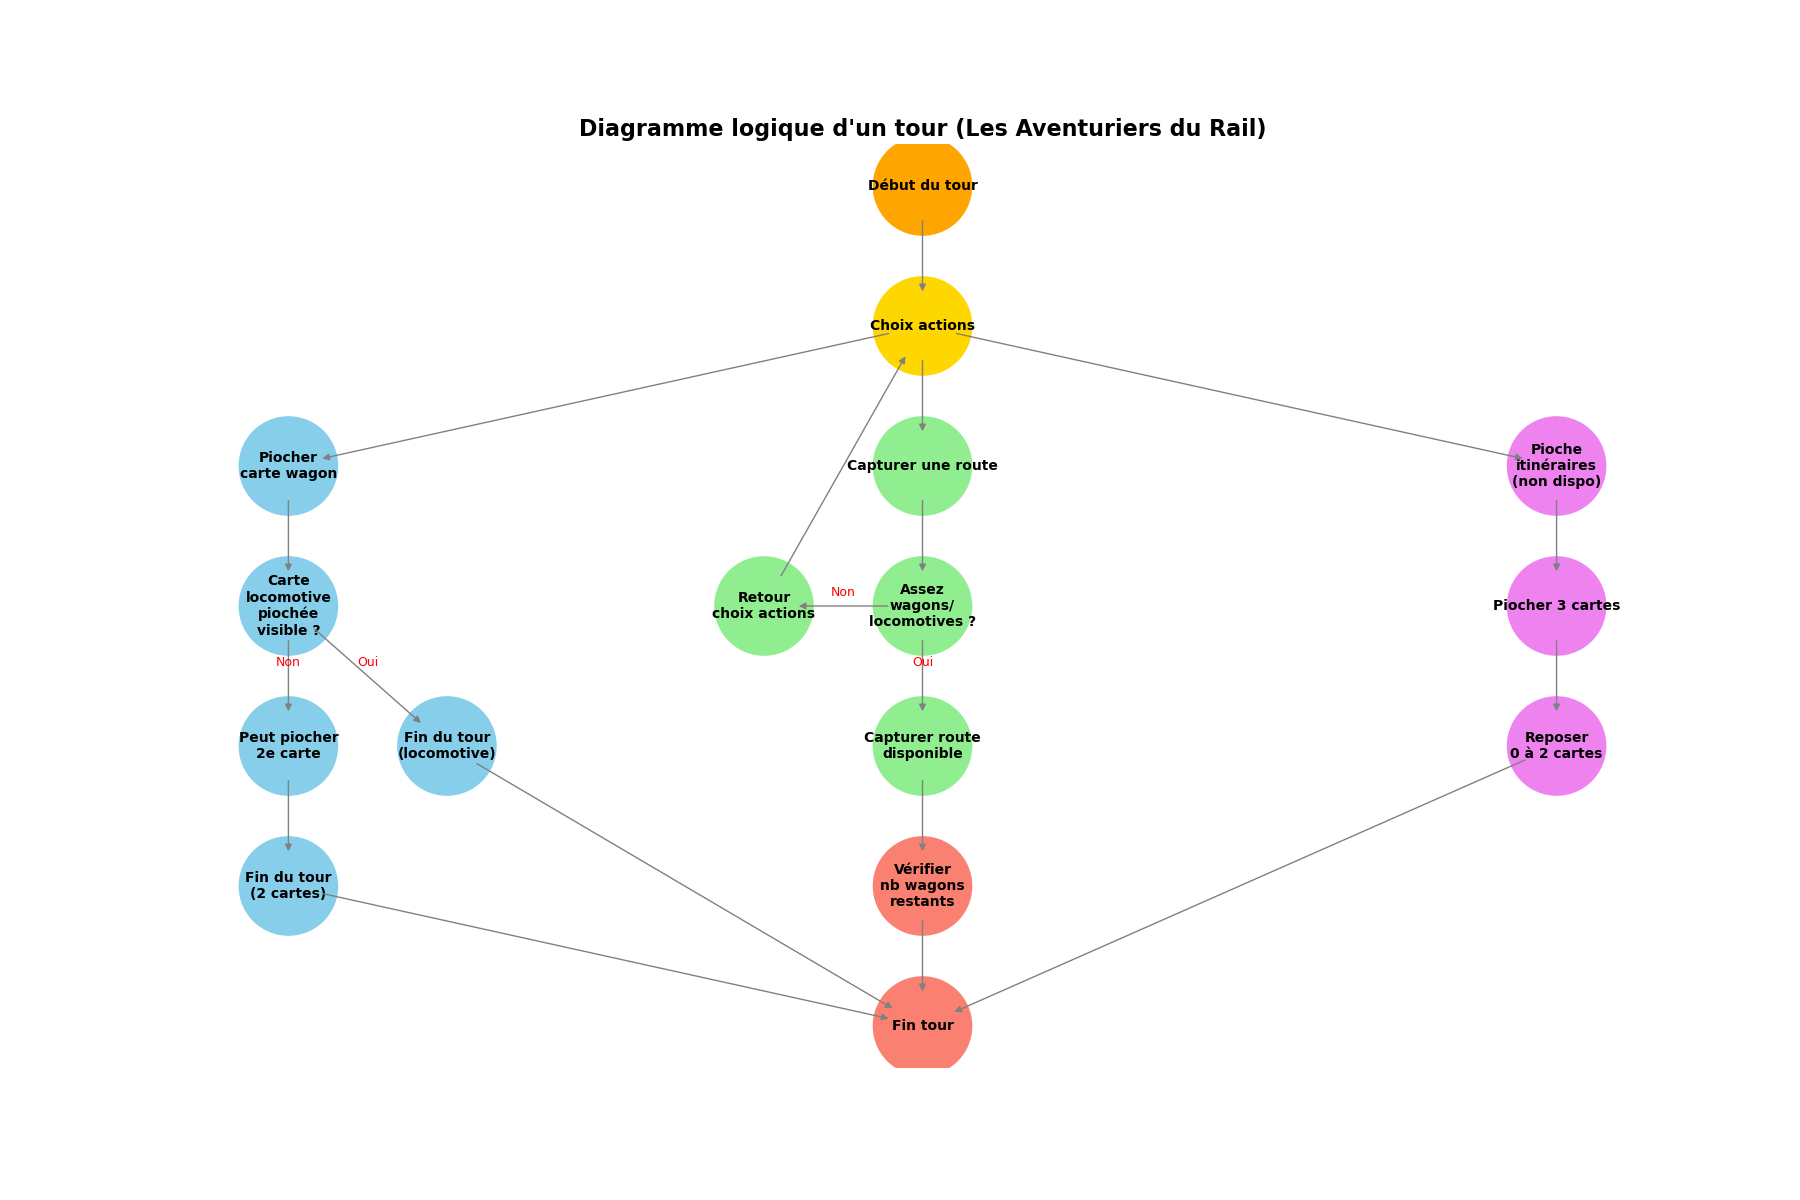
\includegraphics[width=0.9\textwidth]{graph_logique}
    \caption{Schéma du déroulement d’un tour de jeu}
    \label{fig:tour_de_jeu}
\end{figure}

\noindent Ce schéma illustre les choix possibles à chaque tour et les principales conditions vérifiées avant de poursuivre.



\section{Diagramme de classes}

\begin{figure}[H]
    \centering
    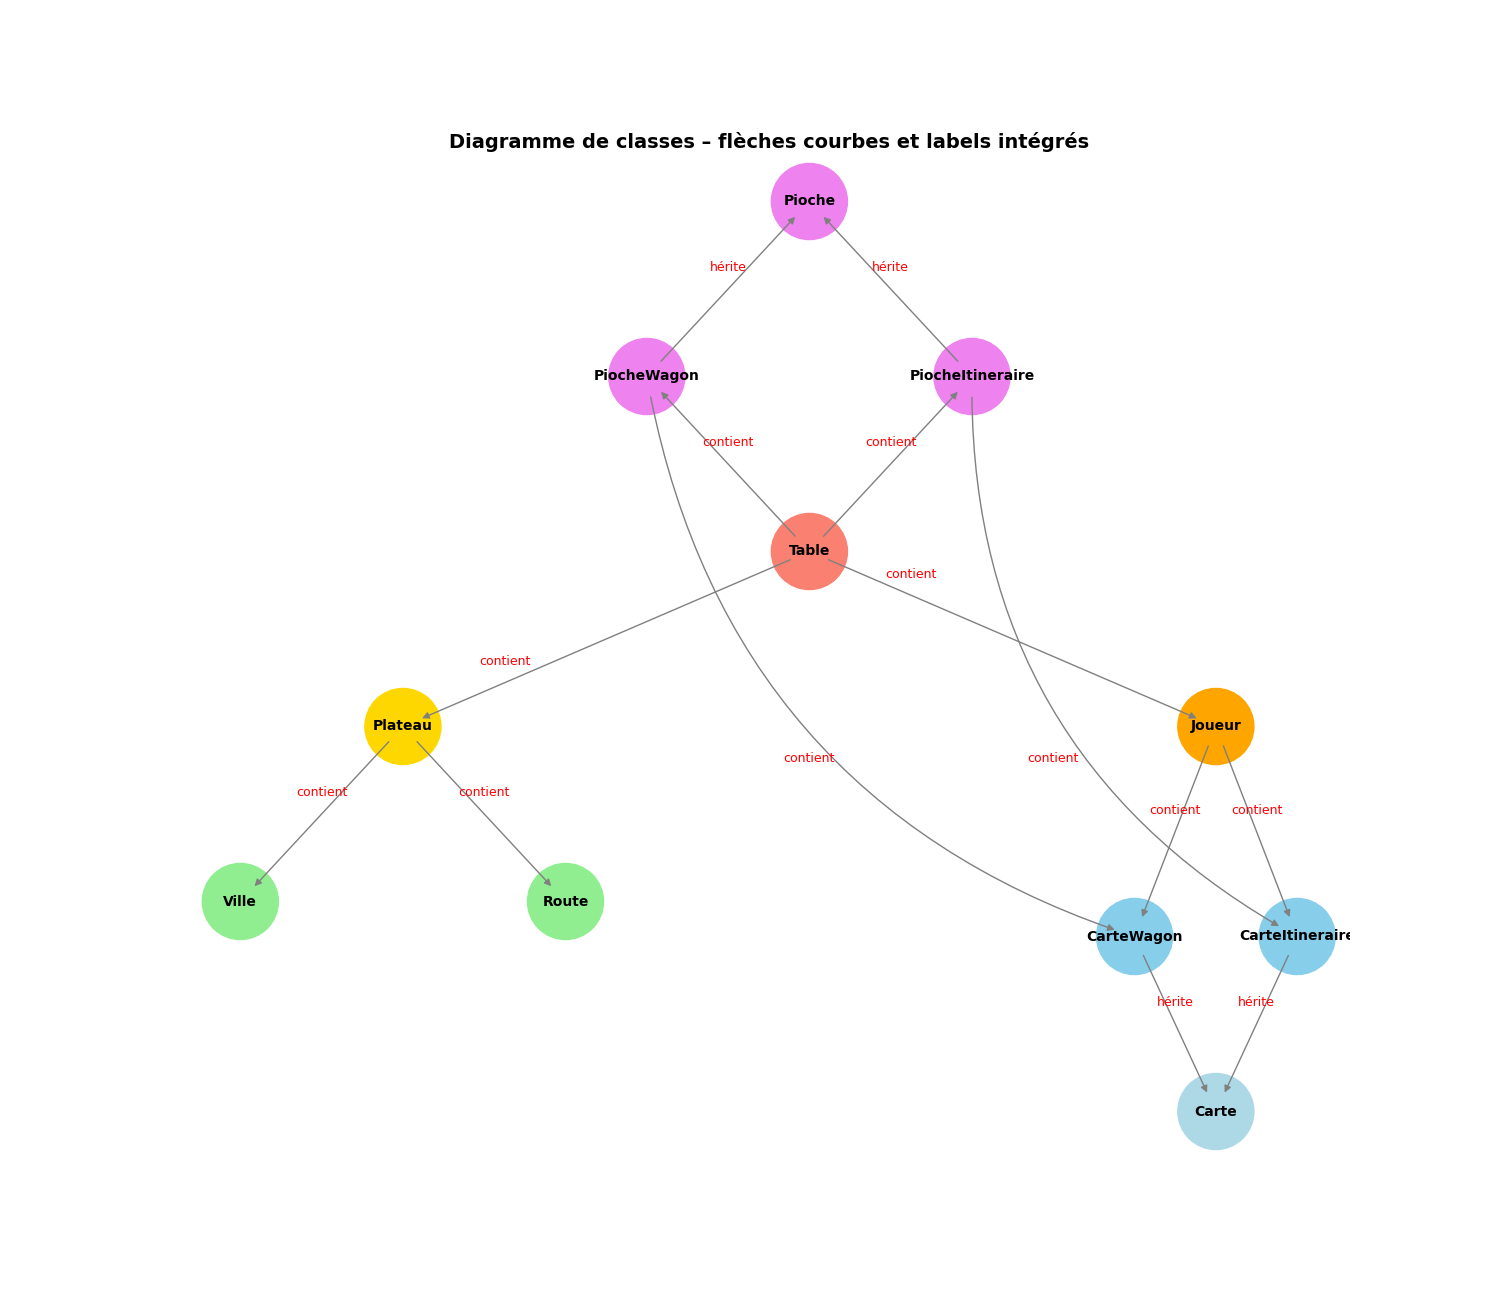
\includegraphics[width=0.9\textwidth]{diagramme_classe}
    \caption{Diagramme de classe}
    \label{fig:diagramme_classe}
\end{figure}


\section{Classes principales}

Le projet repose sur une modélisation orientée objet fidèle à la structure du jeu Les Aventuriers du Rail.
Les principales classes implémentées sont les suivantes :

\subsection*{Classe \texttt{Table}}

Cette classe coordonne la partie. Elle contient l’ensemble des objets nécessaires au déroulement du jeu :
les joueurs, le plateau, les pioches (cartes wagon et cartes itinéraire), ainsi que la gestion des tours.
C’est le point d’entrée principal de l’exécution du jeu.

\begin{itemize}
    \item Initialise les composants de la partie (joueurs, pioches, plateau, objectifs).
    \item Gère le déroulement du jeu tour par tour.
    \item Implémente les règles de pioche, de capture de route, et les contrôles de validité.
\end{itemize}

\subsection*{Classe \texttt{Joueur}}

Un joueur est caractérisé par :
\begin{itemize}
    \item Un nom, un nombre de wagons disponibles.
    \item Une main de cartes wagon et une main de cartes objectif.
    \item Un score évolutif.
\end{itemize}
Le joueur interagit avec la table en piochant, en capturant des routes, et en remplissant ses objectifs.
Des méthodes de jeu automatique seront ajoutées par la suite.

\subsection*{Classe \texttt{Plateau}}

Cette classe représente la carte du jeu, sous forme d’un graphe via \texttt{networkx}. Elle contient :
\begin{itemize}
    \item La liste des villes (sommets du graphe).
    \item La liste des routes entre villes (arêtes, avec couleur et longueur).
    \item Une méthode d'affichage graphique du plateau à l’aide de \texttt{matplotlib}.
\end{itemize}
Elle est utilisée pour déterminer les routes disponibles et afficher l’état du jeu.

\subsection*{Classe \texttt{CarteWagon}}

Cette classe modélise une carte de couleur (ou locomotive). Elle contient :
\begin{itemize}
    \item La couleur de la carte (ex : rouge, vert, locomotive, etc.
\end{itemize}
Elle est utilisée à la fois pour composer la pioche, la main des joueurs, et valider la prise de route.

\subsection*{Classe \texttt{CarteItineraire}}

Une carte objectif contient deux villes et une valeur en points. Elle est attribuée en début de partie.
\begin{itemize}
    \item Les villes sont à relier pour gagner les points.
    \item Si l’objectif n’est pas rempli à la fin, les points sont perdus.
\end{itemize}

\subsection*{Classe \texttt{Ville}}

Une ville est un nœud du graphe du plateau généralement définie par son nom et ses coordonnées graphiques.
Elle est utilisée pour placer les routes sur le graphe et pour calculer les connexions.

\subsection*{Classe \texttt{Route}}

Une route est une liaison entre deux villes. Elle est caractérisée par :
\begin{itemize}
    \item Sa longueur (nombre de wagons nécessaires).
    \item Sa couleur (ou gris pour n’importe quelle couleur).
    \item Le joueur qui l’a capturée (ou \texttt{None} si encore disponible).
\end{itemize}
Elle est représentée par une arête dans le graphe du plateau.

\subsection*{Classes \texttt{PiocheWagon} et \texttt{PiocheItineraire}}

Ces deux classes gèrent respectivement les cartes wagon et les cartes objectif :
\begin{itemize}
    \item Tirage aléatoire.
    \item Cartes visibles pour les wagons.
    \item Règles de pioche (ex : interdiction de piocher une locomotive en 2\up{e} carte).
\end{itemize}

\vspace{1em}
L’ensemble de ces classes interagit selon un principe de composition :
chaque classe possède ses propres données et références vers les objets nécessaires
(ex : \texttt{Table} contient une liste de \texttt{Joueur},une instance de \texttt{Plateau}, etc.).
À ce jour, l’héritage est peu utilisé, mais la structure reste claire et modulaire.


\section{Méthodes importantes}

Certaines méthodes du projet jouent un rôle central dans le déroulement du jeu.
Nous présentons ici celles qui participent directement à l'exécution des actions du joueur et à la mise à jour du plateau.

\subsection*{\texttt{jouer\_tour(joueur)} — classe \texttt{Table}}

Cette méthode coordonne un tour de jeu pour le joueur donné.
Elle appelle selon les cas les fonctions de pioche ou de capture de route, puis actualise le plateau.
Elle gère les règles suivantes :
\begin{itemize}
    \item Choix entre piocher ou capturer une route.
    \item Interdiction de piocher une locomotive en deuxième carte.
    \item Passage au joueur suivant.
\end{itemize}

\subsection*{\texttt{piocher\_cartes\_wagon(joueur)} — classe \texttt{Table}}

Permet au joueur de piocher une ou deux cartes wagon. Elle intègre les règles du jeu :
\begin{itemize}
    \item Le joueur peut choisir parmi les cartes visibles ou tirer à l’aveugle.
    \item Si la première carte est une locomotive visible, le joueur ne peut pas piocher une deuxième carte.
    \item Si le joueur choisit une locomotive en deuxième carte, il est contraint de refaire un choix.
\end{itemize}

\subsection*{\texttt{capturer\_route(joueur)} — classe \texttt{Table}}

Cette méthode permet à un joueur de capturer une route, c’est-à-dire :
\begin{itemize}
    \item Vérifier qu’il possède les cartes nécessaires.
    \item Vérifier qu’il lui reste assez de wagons.
    \item Retirer les cartes utilisées et décrémenter le stock de wagons.
    \item Mettre à jour le plateau : la route devient indisponible et est associée au joueur.
    \item Ajouter les points correspondant à la longueur de la route.
\end{itemize}

\subsection*{\texttt{afficher\_plateau\_graphique()} — classe \texttt{Plateau}}

Affiche dynamiquement l’état du plateau avec les routes et les villes, en utilisant la bibliothèque \texttt{matplotlib}.
Cette méthode est utile :
\begin{itemize}
    \item Pour visualiser les routes encore disponibles.
    \item Pour observer les routes capturées par chaque joueur.
    \item Pour intégrer une première forme d'IHM dans le projet.
\end{itemize}

\subsection*{Méthodes à venir}

D'autres méthodes clés seront développées dans la suite du projet :
\begin{itemize}
    \item Calcul automatique des objectifs réussis (via composantes connexes).
    \item Détection du plus long chemin (bonus de 10 points).
    \item Gestion du joueur automatique.
    \item Mise à jour des cartes visibles en cas d'excès de locomotives.
\end{itemize}



\chapter{Figures imposées}
\addcontentsline{toc}{chapter}{Figures imposées}

Le projet respecte plusieurs des figures imposées, réparties en deux catégories :
les six figures communes à tous les sujets, et trois figures supplémentaires sélectionnées par le binôme.

Nous listons ci-dessous ces figures, en distinguant celles qui sont clairement implémentées,
celles qui restent à travailler, et celles qui ne sont pas pertinentes dans le cadre de notre projet.

\section*{1. Figures imposées communes à tous les sujets}

\begin{itemize}
    \item \textbf{Création d’au moins quatre types d’objets avec variables d’instance} – \underline{Implémentée} \\
    Le projet comprend les classes suivantes : \texttt{Table}, \texttt{Joueur}, \texttt{Plateau}, \texttt{CarteWagon},
    \texttt{CarteItineraire}, \texttt{Ville}, \texttt{Route}.
    Chacune dispose de plusieurs variables d’instance décrivant leur état propre.

    \item \textbf{Structuration du code en plusieurs modules} – \underline{Partiellement implémentée} \\
    Le code principal est actuellement regroupé dans un fichier unique
    (\texttt{LesAventuriersDuRail.py}), mais un second module est dédié au diagramme de classes (\texttt{Diag\_classe.py}).
    Une restructuration en plusieurs modules thématiques (cartes, joueurs, plateau, etc) est prévue pour la version finale.

    \item \textbf{Héritage / composition entre au moins trois types} – \underline{Partiellement implémentée} \\
    Le code repose principalement sur la \textbf{composition}
    (ex. : \texttt{Table} contient un \texttt{Plateau}, des \texttt{Joueur}, des pioches, mais aucun héritage n'est actuellement utilisé.
    Il n’y a pas de classe abstraite de type \texttt{Carte}, ou \texttt{Pioche}.
    Cette figure sera retravaillée pour introduire un héritage minimal pertinent.

    \item \textbf{Documentation et commentaires du code} – \underline{En cours} \\
    Des docstrings explicatifs sont en cours d’ajout pour chaque classe et méthode.
    Le champ \texttt{:author:} est prévu pour identifier les contributeurs.
    Une documentation complète est prévue pour la livraison finale.

    \item \textbf{Tests unitaires (au moins 4 méthodes, 2 cas chacune)} – \underline{À développer} \\
    Les tests unitaires sont à formaliser.
    Les fonctions clés (\texttt{piocher\_cartes\_wagon}, \texttt{capturer\_route}, etc.) ont été testées manuellement,
    mais pas encore via un framework comme \texttt{pytest}.
    Ce point sera prioritaire pour l’étape suivante.

    \item \textbf{Stockage de données (fichier ou BDD)} – \underline{Non implémentée} \\
    À ce jour, aucune lecture ou écriture de fichier n’est réalisée.
    Cette figure ne semble pas essentielle dans notre sujet actuel, car la partie sauvegarde/chargement n’est pas exigée dans les objectifs pédagogiques.
    Elle pourrait être utilisée en option pour mémoriser l’état du plateau ou une configuration.

\end{itemize}

\section*{2. Figures supplémentaires choisies pour le sujet}

\begin{itemize}
    \item \textbf{Algorithme d’optimisation} – \underline{À venir} \\
    Un joueur intelligent (objectif 4) est prévu.
    Il devra construire un sous-graphe reliant ses objectifs en minimisant le nombre d’arêtes ou de couleurs utilisées.
    Cette tâche est liée à un problème d’arbre de Steiner et constitue un bon candidat pour l’optimisation.

    \item \textbf{Fonction récursive} – \underline{Non encore utilisée} \\
    Aucune fonction récursive n’est présente pour le moment.
    Elle pourrait être introduite dans le calcul du plus long chemin (bonus de 10 points), via une exploration récursive du graphe de routes du joueur.

    \item \textbf{Exploration de graphe avec bibliothèque dédiée} – \underline{Implémentée} \\
    Le projet utilise \texttt{networkx} pour représenter et manipuler le graphe du plateau.
    Cela inclut la détection des routes disponibles, la suppression d’arêtes, l’évaluation des composantes connexes.
    Cette figure est donc clairement remplie.

\end{itemize}

\section*{3. Figures non pertinentes dans le cadre de ce projet}

Les figures suivantes ne sont pas jugées pertinentes dans notre cas :

\begin{itemize}
    \item \textbf{Calcul vectoriel} : non applicable, car le projet ne traite pas de données vectorielles ou numériques en masse.
    \item \textbf{Design patterns type}

\end{itemize}

\chapter{Tests et résultats}

\section{Méthodes testées manuellement}
%% ➤ Jouer un tour, piocher des cartes, capturer une route, attribution initiale…

\section{Tests à implémenter}
%% ➤ Tests unitaires avec pytest pour : piocher, capturer, fin de partie, erreur de joueur, etc.

\chapter{Avancement des objectifs}

%% ➤ Reprendre ici le tableau ou texte déjà rédigé avec Objectifs 1 à 4 + IHM.
%% ➤ Dire ce qui est fait / partiel / à venir.

\chapter{Perspectives et améliorations}

%% ➤ Découpage du code en modules
%% ➤ Implémentation du joueur aléatoire
%% ➤ Calcul des scores (objectif + composante connexe)
%% ➤ Plus long chemin
%% ➤ Joueur intelligent avec graphe de routes
%% ➤ Interface plus interactive (optionnelle)

\chapter*{Conclusion}
\addcontentsline{toc}{chapter}{Conclusion}

%% ➤ Résumer ce qui est déjà fait
%% ➤ Dire ce que vous avez appris techniquement
%% ➤ Présenter les priorités pour la 2ᵉ étape

\appendix

\chapter{Annexes}


%% ➤ lien github, README, extrait de codes utiles,

\end{document}